\section{The Anonymous Face Tracking Panda}
As previously stated, living with a mental illness can be isolating and the stigma around mental health issues makes people hesitant to seek professional help. The primary purpose of this thesis is to create a functional prototype capable of connecting people with mental health specialists anonymously, while still maintaining patient-therapist empathy.

\subsection{Approach}
A working prototype was developed using Unreal Engine Blueprints (a node-based interface to create gameplay elements), the UE4, Metahumans, and Live Link connected to an iPhone's camera. In the prototype, patients can communicate with mental health specialists via video conferencing anonymously, as patient's smartphone functions as a virtual camera that allows the mental health practitioner to see the patient's facial expressions in real-time via a virtual avatar.

Using an Apple device with the TrueDepth sensor and the Live Link Face app, one can capture numerous facial tracking points by creating a depth map of ones’ face while projecting and analyzing over 30,000 invisible dots, as well as capturing an infrared face image. The data collected by the Apple device and app is delivered to the UE4 environment via a directed internet connection maintained between the user's iPhone/iPad and the Unreal Engine. When data is received by Unreal Engine 4, it is evaluated and turned into VA movements via Live Link Plugin, as shown in Figure \ref{fig:facialExpressions} and Figure \ref{fig:blueprintsData}.

\begin{figure}[!htb]
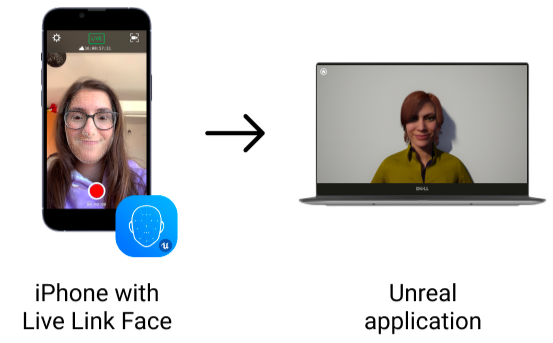
\includegraphics[width=0.7\textwidth]{figures/howItWorks.png}
\centering
\caption{How the facial expressions are captured and represented}
\label{fig:facialExpressions}
\end{figure}

\begin{figure}[!htb]
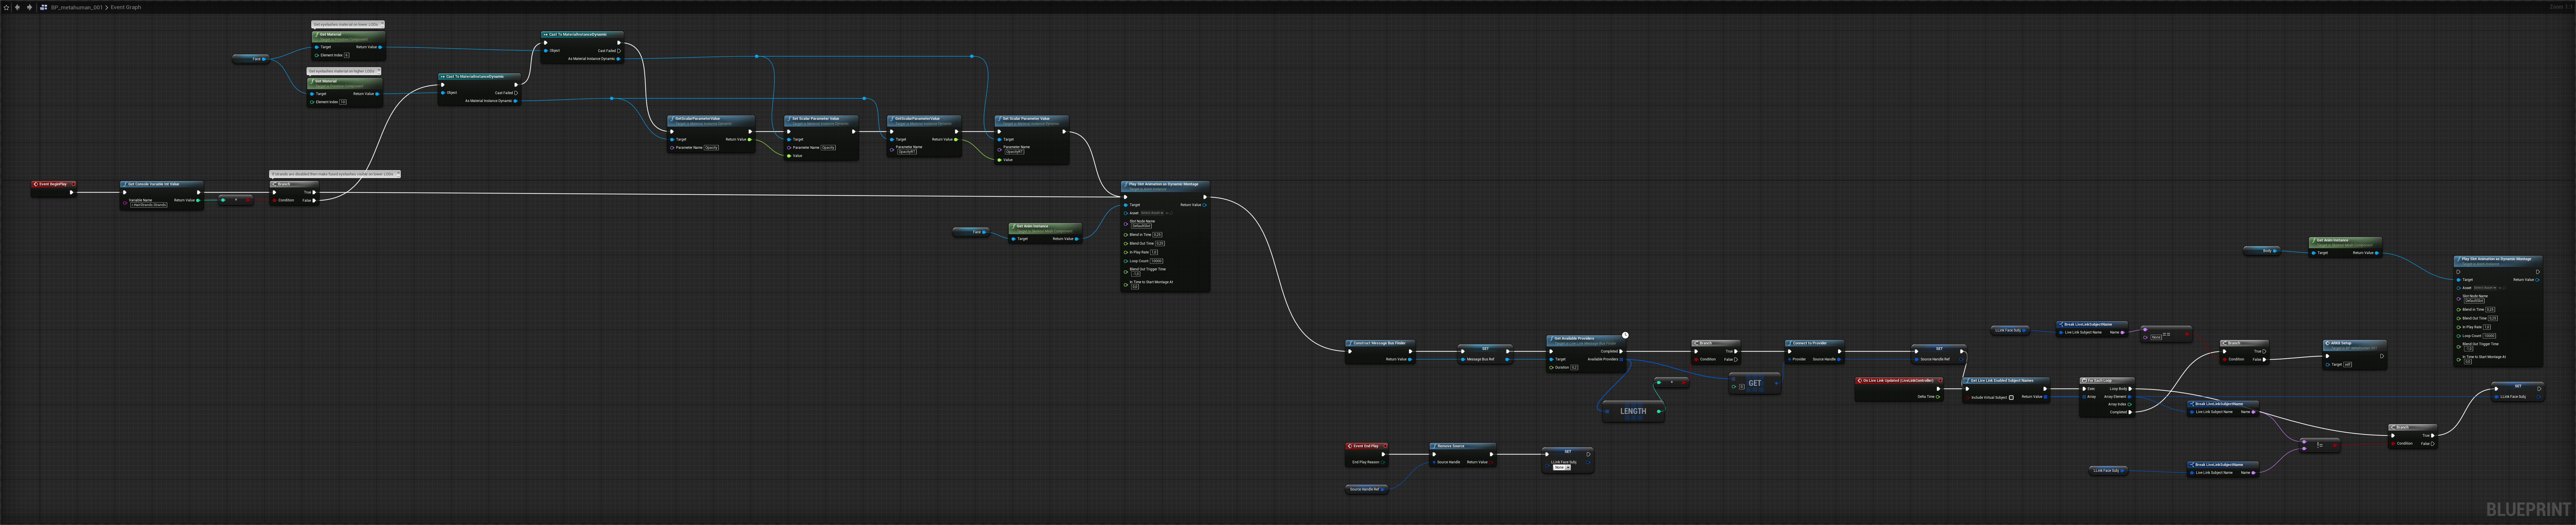
\includegraphics[width=\textwidth]{figures/hereItBegins.png}
\centering
\caption{Blueprints responsible for the connection and stream of data}
\label{fig:blueprintsData}
\end{figure}

The goal of the Live Link Plugin \cite{EPI22} is to provide a unified interface for streaming and consuming animation data into Unreal Engine 4 from one or more external sources, such as Display Data Channel (DDC) tools or Mocap Servers. It's built to be extensible via Unreal Plugins, allowing third parties to create new features without having to make and maintain Engine changes. Live Link can also be used by Motion Capture Systems to stream data into the Engine that can be previewed in real time.

To provide users with options, and thus reach a wider audience, four metahumans (two males and two females, of different ethnicities) were exported from the Metahuman Creator \cite{EPI21}, and the Quixel Bridge application into UE4, where, in order to make the interaction with the prototype easier, a minimalist user interface (Figure \ref{fig:screenshotApp}) was created that allows users to choose their preferred avatar. 

\begin{figure}[!htb]
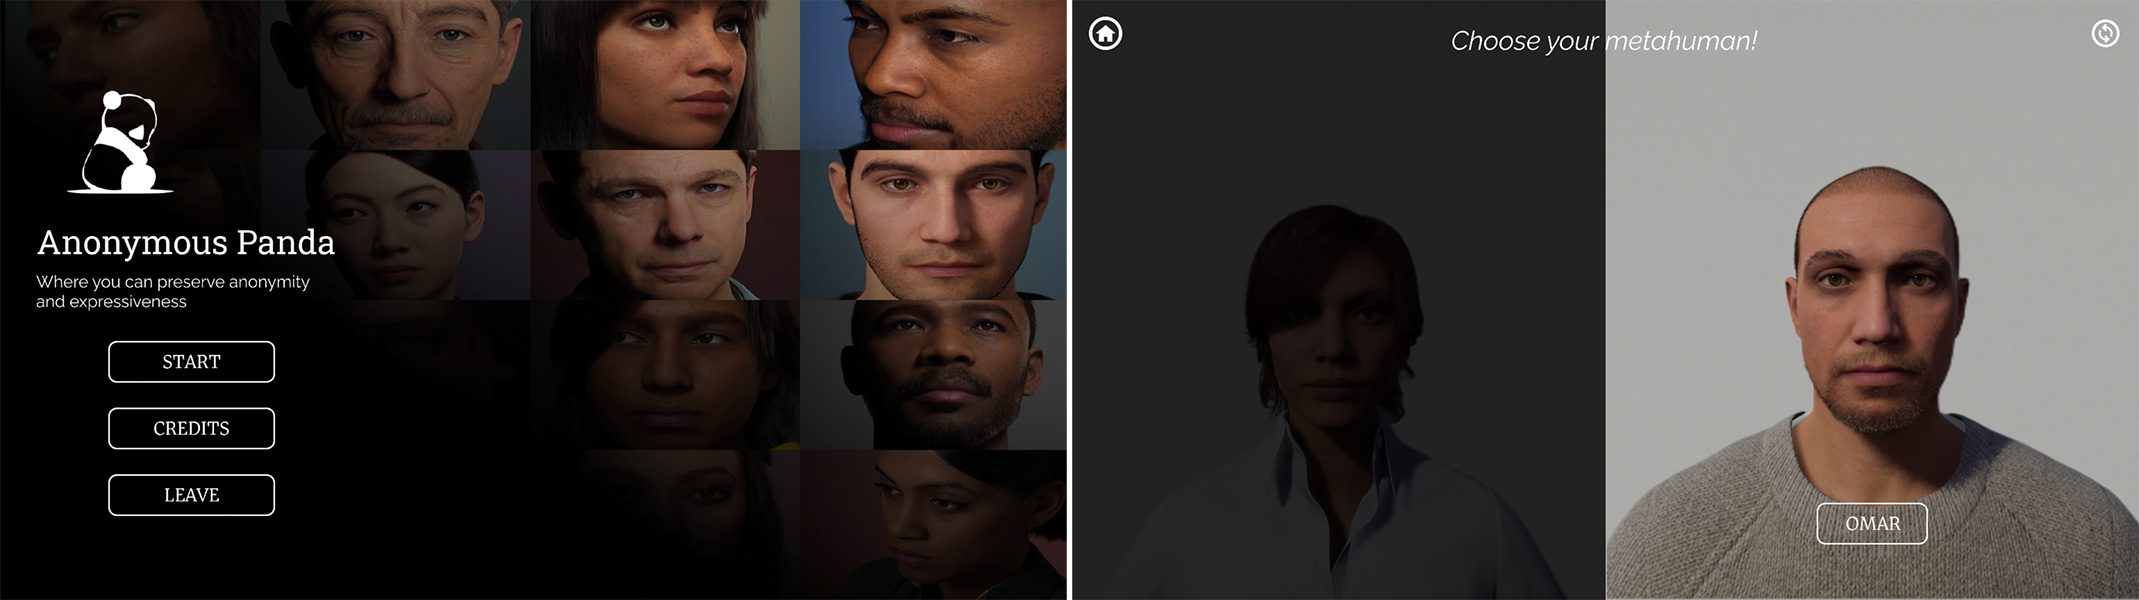
\includegraphics[width=\textwidth]{figures/ui-app.jpg}
\centering
\caption{Screenshots of the Anonymous Panda application}
\label{fig:screenshotApp}
\end{figure}

Although custom metahumans were not employed in this version of the prototype, due to performance and optimization concerns, the chosen metahumans (Figure \ref{fig:metahumans}) were pre-made by Epic Games and available on Quixel Bridge. These concerns were alleviated by using these four metahumans because Epic Games pre-defines export settings and assets compatible with many devices.

\begin{figure}[!htb]
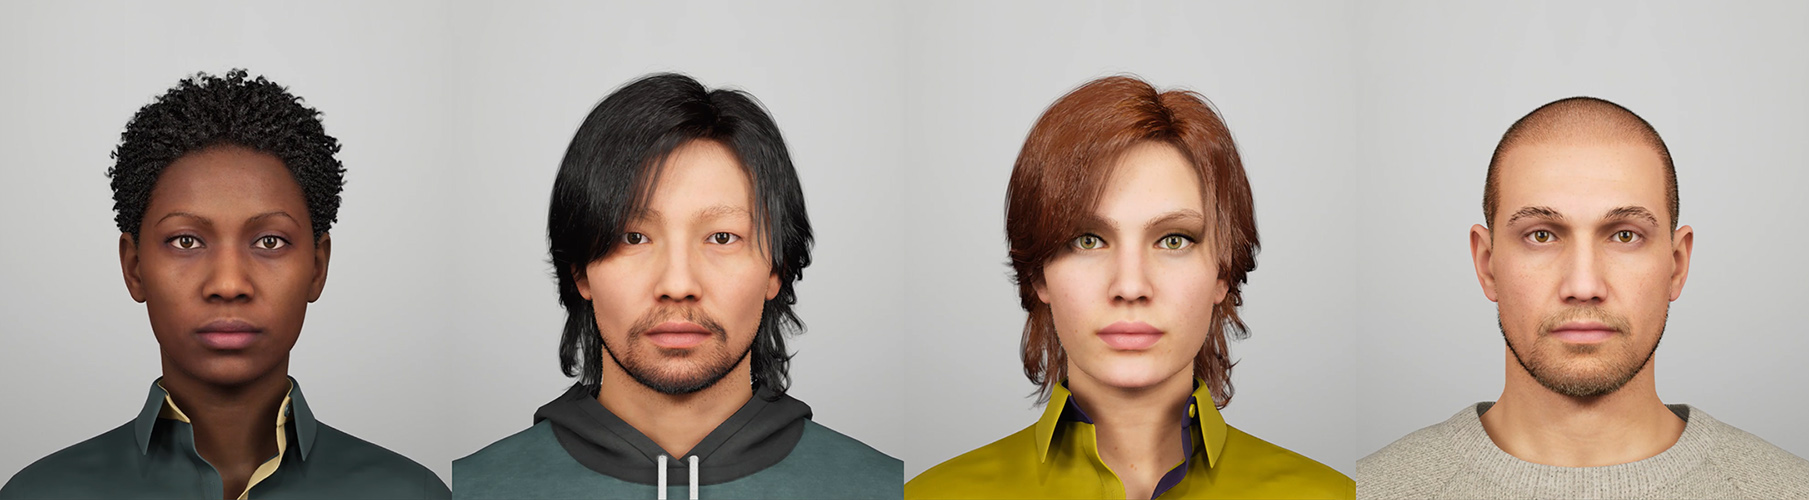
\includegraphics[width=\textwidth]{figures/4metahumans.jpg}
\centering
\caption{The current metahumans used on the prototype}
\label{fig:metahumans}
\end{figure}

As the human face is the primary means of non-verbal communication \cite{MALO20, KUJ03, SAU19}, it is typically used to communicate a person's emotions and mood and to provide visual cues to a person's physical state. Facial expressions are easily distinguished across cultures and automatically perceived so that we can immediately evaluate someone's emotional state. As Figure \ref{fig:metahumanFacialExpressions} makes visible, the facial expression of the VA are perceptible in the current version of the prototype. 

\begin{figure}[!htb]
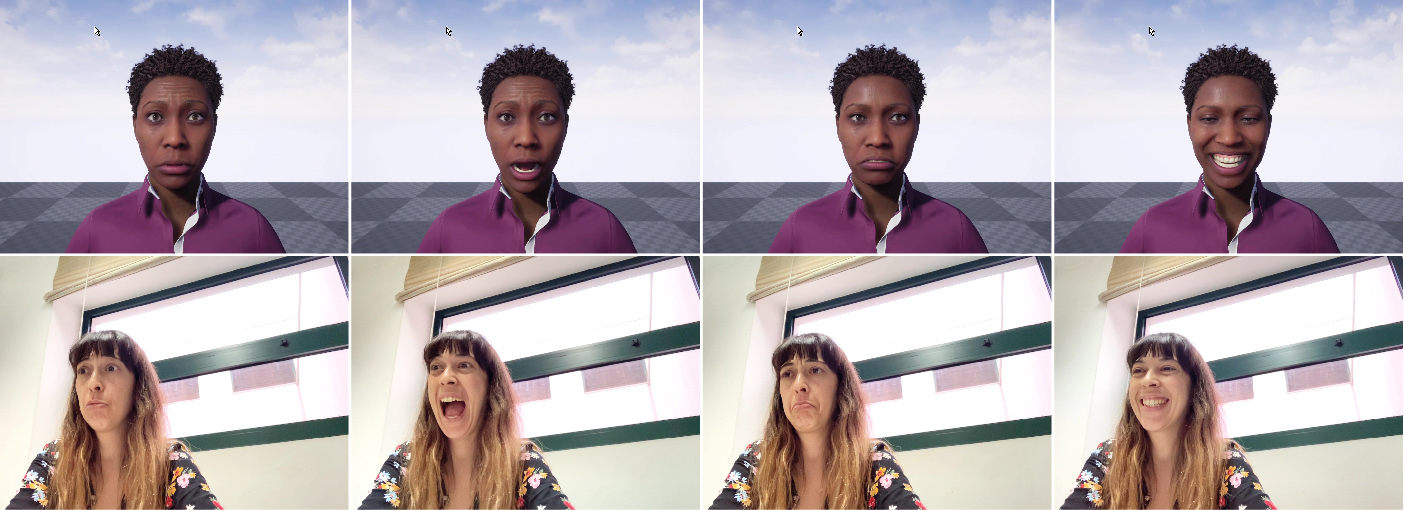
\includegraphics[width=\textwidth]{figures/expressionTest.jpg}
\centering
\caption{Examples of facial expressions and their virtual avatar depiction}
\label{fig:metahumanFacialExpressions}
\end{figure}

However, upon a closer look, even though the avatar could accurately represent the user's facial expressions using the default functions of the live link plugin, a minor flaw in terms of lip positioning was found, particularly when the mouth should be closed or when the user was trying to express a negative emotion (e.g., sadness). To solve this issue, the upper lip values were slightly adjusted (Figure \ref{fig:blueprintAnimation}) before being reconverted to metahuman animation.

\begin{figure}[!htb]
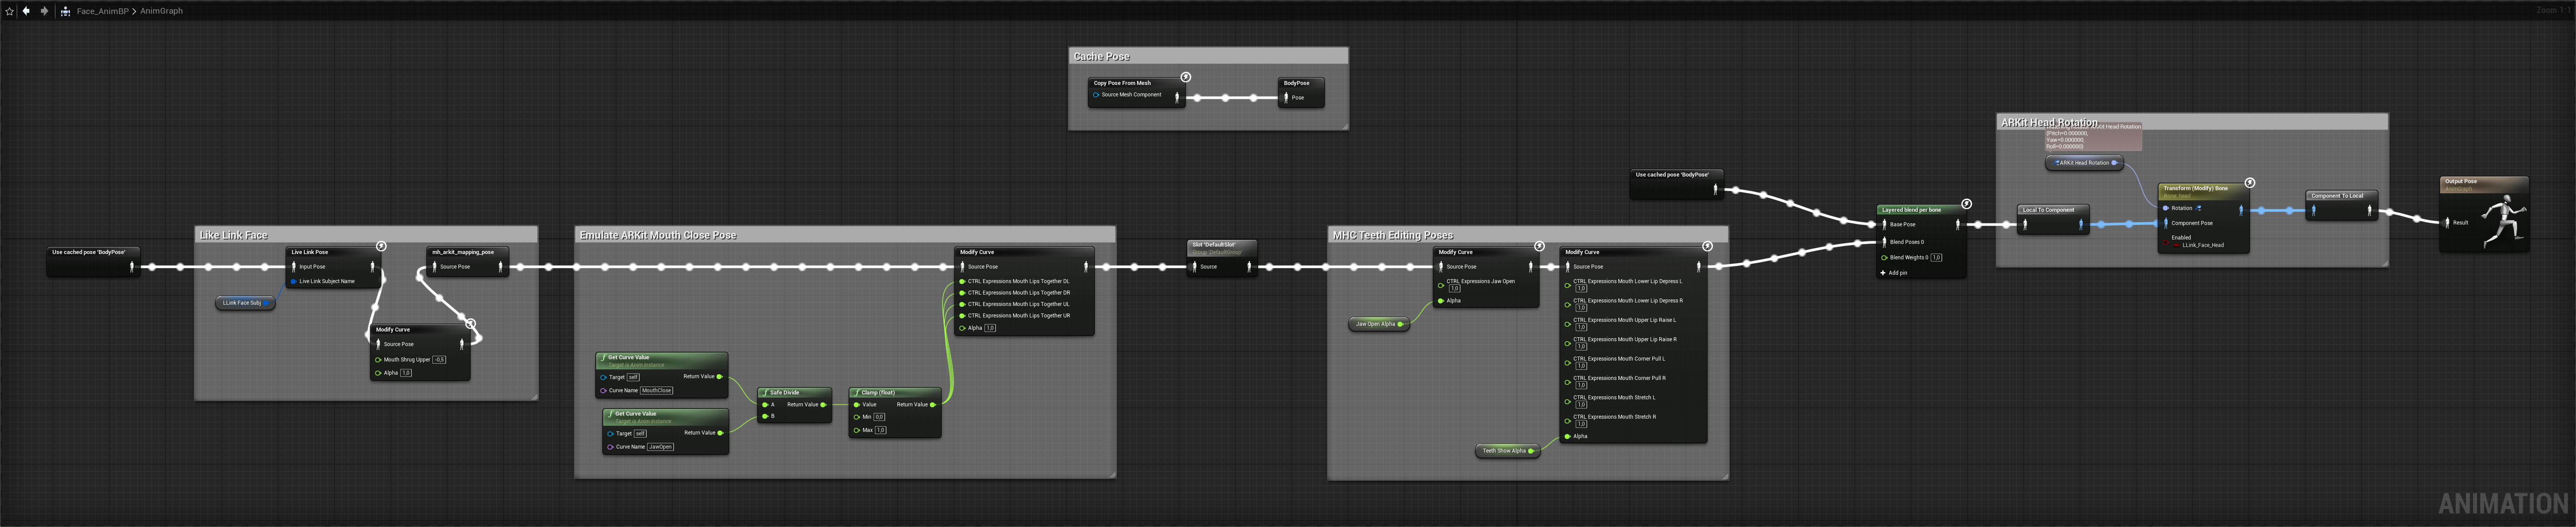
\includegraphics[width=\textwidth]{figures/facialConfig.png}
\centering
\caption{Blueprints responsible for the conversion of data to animation of metahuman}
\label{fig:blueprintAnimation}
\end{figure}

Although one of the foundations of this thesis is patient-therapist communication,  the current prototype requires the user to share only the UE4 application as if it were a webcam, which necessitates the usage of a video conferencing tool as well as OBS Studio Virtual Camera, a live streaming tool (Figure \ref{fig:prototype} and \ref{fig:obs}). Even though this causes a slight delay, it can be used in a video conference.

\begin{figure}[!htb]
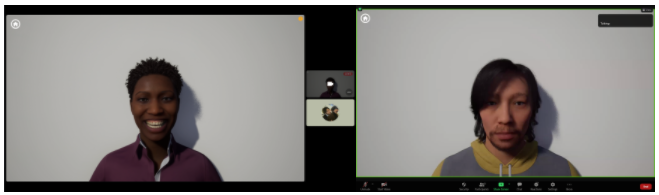
\includegraphics[width=\textwidth]{figures/zoomAndDiscord.PNG}
\centering
\caption{The prototype in use on a call via Discord and Zoom}
\label{fig:prototype}
\end{figure}

\begin{figure}[!htb]
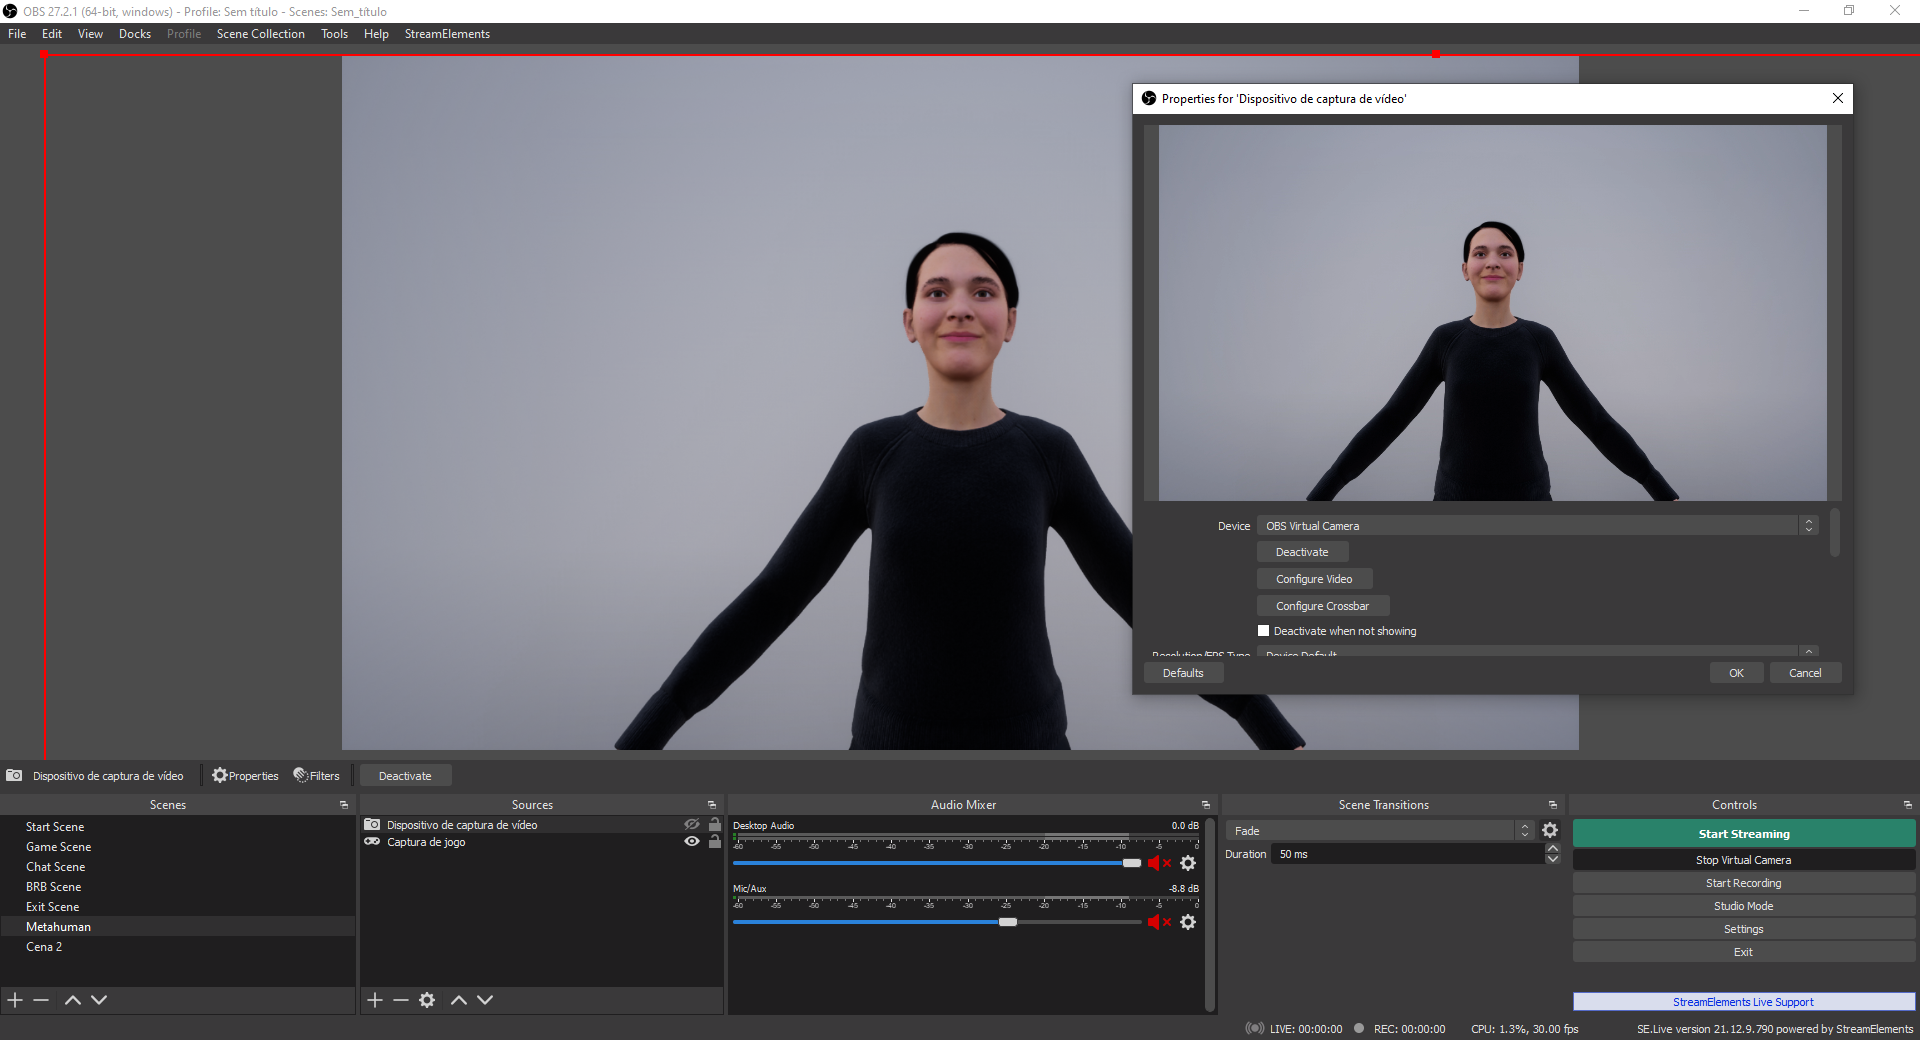
\includegraphics[width=\textwidth]{figures/streamingTool.PNG}
\centering
\caption{Virtual Camera setup on OBS Studio}
\label{fig:obs}
\end{figure}

\subsubsection{Limitations}
One of the thesis's challenges is to use customized models because these models demand a lot of optimization. After all, they are resource-intensive, limiting the patient's expressions from being viewed clearly and fluidly. 

Nonetheless, the creation and use of custom metahumans has already improved thanks to recent contributions from Epic Games. However, because many assets are still in development, the design and use of metahumans are still limited. Meaning, if these assets are excluded, it should be possible to use metahumans other than those pre-defined by Epic Games. Figure \ref{fig:metahumanWarning} shows a warning about using a metahuman with groom elements under development, as well as a warning for only displaying it in Level of Detail (LOD) 0 and 1. The many levels that make up each groom element's LODs set, which includes hair, mustache, beard, eye brows, eye lashes, and vellus (also called peach fuzz), are depicted in Figure \ref{fig:LOD}.

\begin{figure}[!htb]
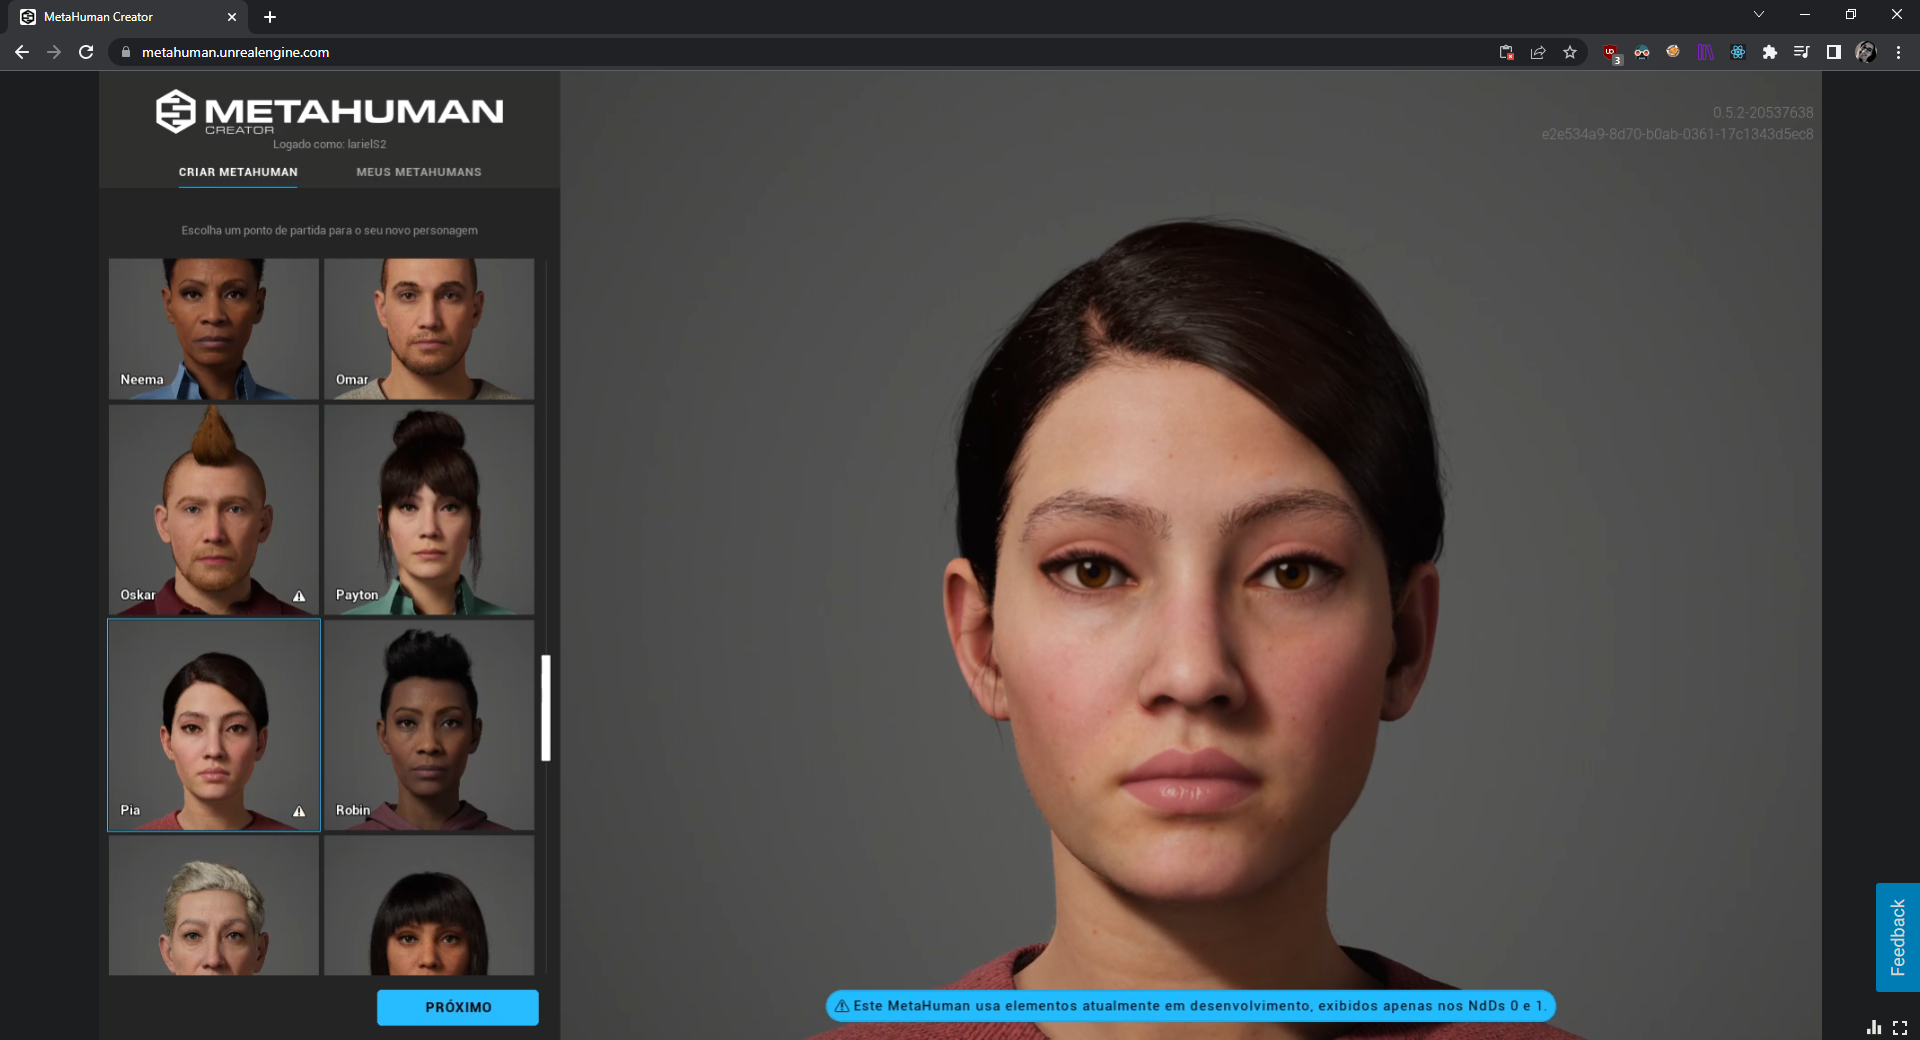
\includegraphics[width=\textwidth]{figures/warningMetahumanCreator.PNG}
\centering
\caption{Metahuman Creator warning for elements under development}
\label{fig:metahumanWarning}
\end{figure}

\begin{figure}[!htb]
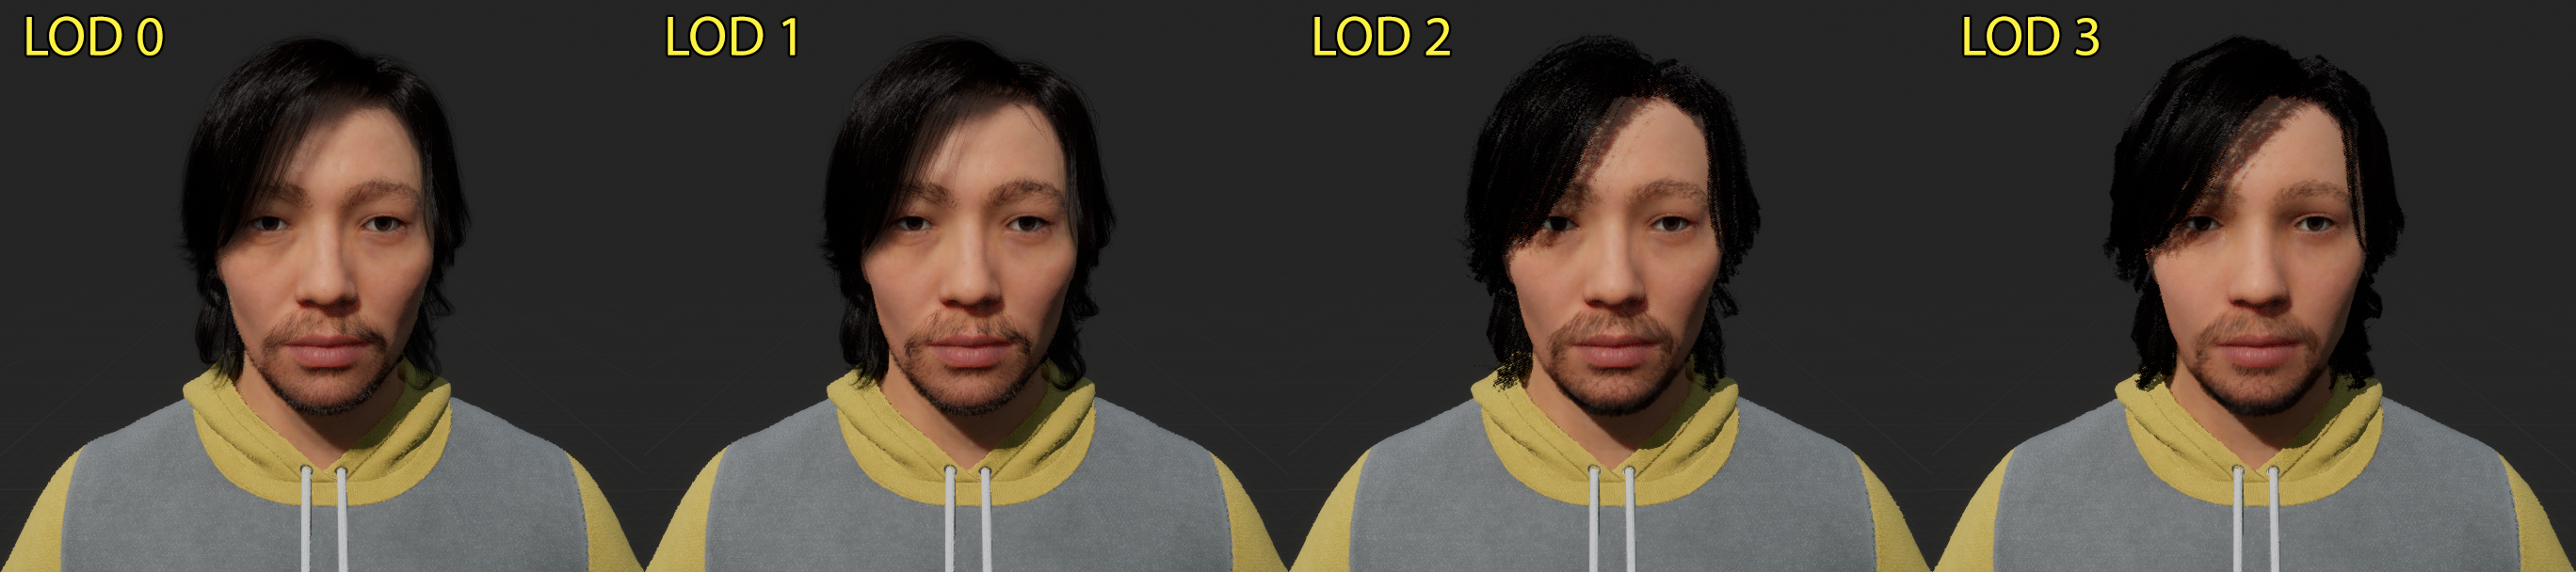
\includegraphics[width=\textwidth]{figures/GroomLODSequence1.PNG}
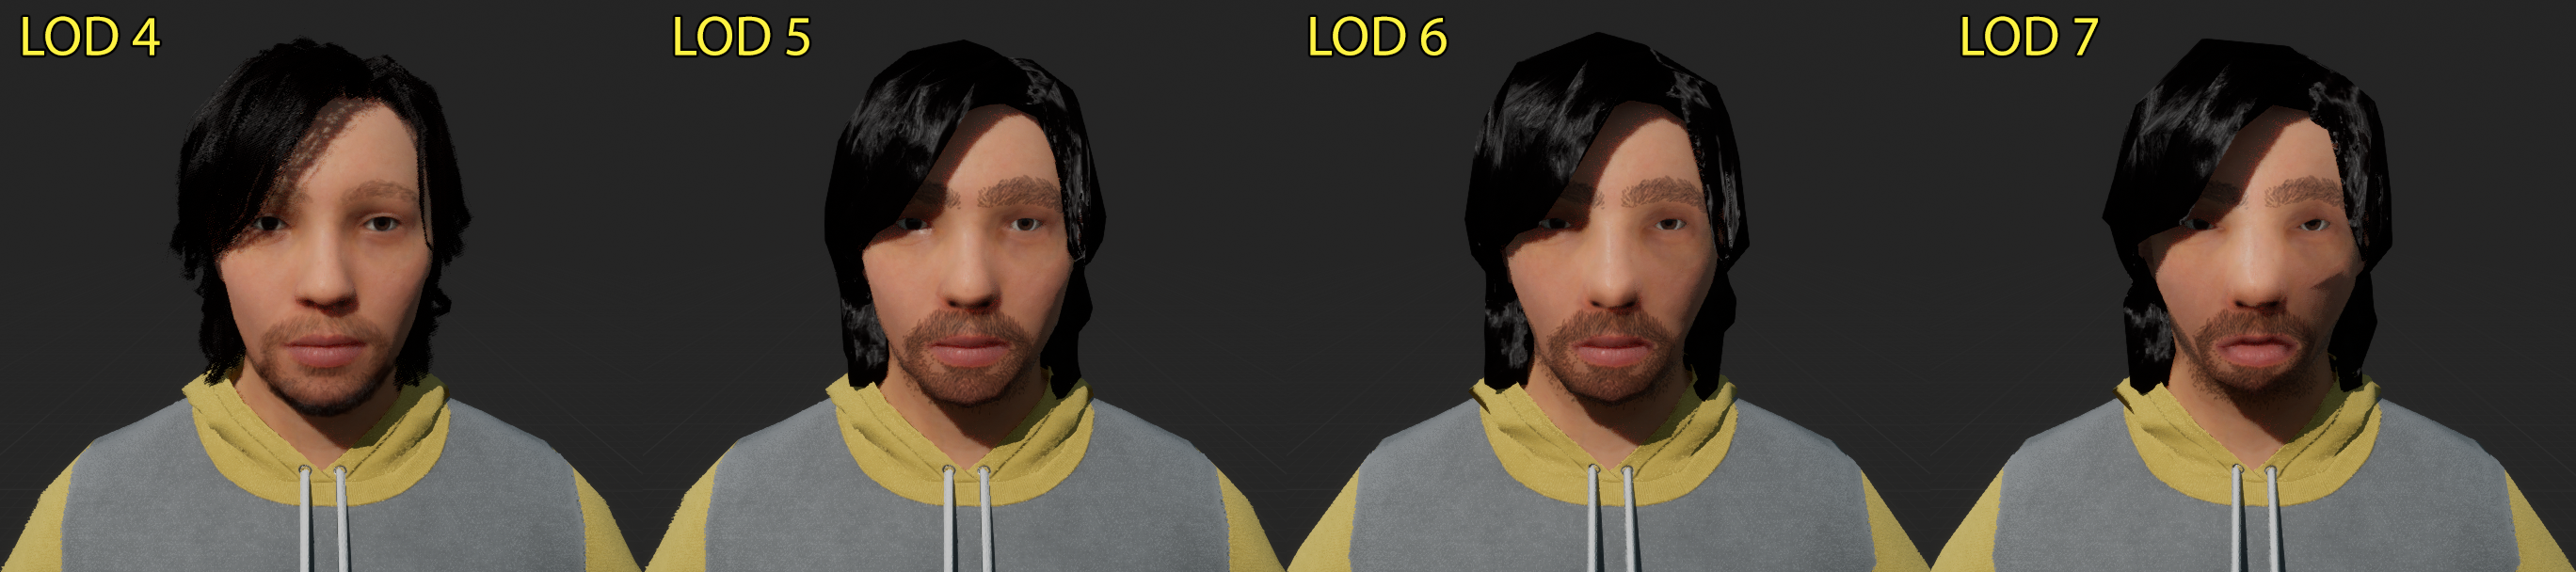
\includegraphics[width=\textwidth]{figures/GroomLODSequence2.PNG}
\centering
\caption{Groom LoD sequence from cinematic (0) to the lowest (7) quality}
\label{fig:LOD}
\end{figure}

Moreover, because this is a resource-intensive application, another difficulty is how people will utilize it. As a result, one of the problems is figuring out how to develop this program to reach everyone who needs it. 

Finally, in order to assess the feasibility of this approach, the following methodology was employed.

\subsection{Methodology}
To assess the feasibility of the previously described approach and test user's empathy with the metahumans, a controlled experiment will test whether this virtual avatars are able to convey the same emotional depth as a real person (\textbf{RQ\textsubscript{1}}).

\makebox[\textwidth]{\color{orange} * IN PROGRESS *}

Table \ref{tab:dataset} summarizes the information about each dataset.

\begin{table}[!htb]
    \centering
	\begin{tabular*}{0.8\linewidth}{ @{\extracolsep{\fill}} lcr}
		\hline
		\small Year of data collection  & \small & \small 2022\\
        \small Participants (\textit{N})  & \small & \small 48\\
		\hline
		
        \multicolumn{3}{c}{Collected data}\\
		\small Demographic Data  & \small & \small Yes\\
        \small Baseline Empathy Levels  & \small & \small Yes\\
        \small Cognitive and Affective Empathy Levels  & \small & \small Yes\\
        \hline
		
        \multicolumn{3}{c}{Usage in this study}\\
        \small\textbf{RQ\textsubscript{1}} (emotional response)  & \small & \small Yes\\
        \small\textbf{RQ\textsubscript{2}} (verbal self-disclosure)  & \small & \small No\\
		
		\hline\\
	\end{tabular*}
	\caption{Summary of the datasets used in study one}
	\label{tab:dataset}
\end{table}

\subsubsection{Participants}

\makebox[\textwidth]{\color{red} * TO-DO *}

\subsubsection{Procedure}

\makebox[\textwidth]{\color{red} * TO-DO *}

\subsubsection{Hypotheses and Analyses}
To answer \textbf{RQ\textsubscript{1}} (Can virtual avatars elicit the same emotional response as human-to-human interactions?), we tested if our independent variable stimuli --- which has three levels, metahuman (G\textsubscript{1}), real person (G\textsubscript{2}), and transcript (G\textsubscript{3}) --- had an effect on participants' cognitive and affective empathy. Because the participants' CE and AE are supposed to indicate if the feelings and emotions conveyed via stimuli were understood, it's reasonable to assume that those with greater baseline empathy levels would comprehend the feelings and emotions better.

Therefore, our hypotheses were:

\textbf{\textit{H}\textsubscript{1}} - All stimuli conditions can elicit cognitive emotion in their respective groups.

\textbf{\textit{H}\textsubscript{2}} - The metahuman video stimuli elicit more affective empathy than the person video stimuli.

\textbf{\textit{H}\textsubscript{3}} - The person video stimuli elicit more affective empathy than the transcript stimuli.

\makebox[\textwidth]{\color{orange} * IN PROGRESS *}

% The game name is a categorical variable, which we can use to group game mentions. Thus, to test H1–H3, we needed to test if the scores of the player traits, game elements, and game playing styles were significantly different per group. This required a multivariate analysis method because each one of these constructs is represented by more than one score. However, it was not possible to use a multivariate analysis of variance (MANOVA) because our data violated the assumptions of normality (verified with the Kolmogorov-Smirnov test) and homogeneity of variances (verified with Levene’s test). Therefore, we used the npmv package (Nonparametric Comparison of Multivariate Samples, v. 2.4.0; [23]) for the statistical software R (v. 3.5.2, 2018), which uses rank-based approaches to test the overall null hypothesis (see [9, 10] for the underlying theory). The package calculates four different test statistics, which all consistently led to the same results in our tests. Thus, we chose to report only the Wilks’ Lambda (λ) type test statistics [52] because it is the default one to use according to the package’s manual [23]. After verifying the overall significance of each relationship, we followed up with one-way Kruskal-Wallis (KW) tests on SPSS (v. 23, IBM, 2015) to find out which individual types of scores were significant. Additionally, we calculated the effect size η 2 from the KW test statistic H (see [26, 33]) and produced charts to easily compare the median scores per game.

The retrieved data was analyzed in the IBM SPSS statistics software, using a statistical significance level of 0.05.
A Kruskal-Wallis H test was used for ordinal, nonparametric data to assess whether there were any statistically significant differences between the 3 conditions in terms of cognitive and affective empathy. A Mann-Whitney U test was also performed to compare if there were differences in social presence between the metahuman and the real person video conditions.

\subsubsection{Results}

\makebox[\textwidth]{\color{red} * TO-DO *}

\subsubsection{Discussion}

\makebox[\textwidth]{\color{red} * TO-DO *}